在现代计算机中,为了便于软件移植,一般均采用\textbf{IEEE
754标准}来表示浮点数。在介绍IEEE
754标准前,有必要先介绍一下浮点数的表示形式。

既然尾数和阶码分别是定点小数和定点整数,即尾数和阶码都是有符号位的,那么就可以写出\textbf{浮点数N的一般格式},如图2-1所示。

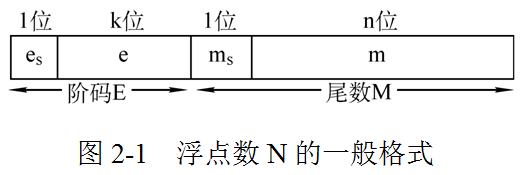
\includegraphics[width=2.70833in,height=0.89583in]{png-jpeg-pics/6FE5A2B6C1359E9800E06FB67C945377.png}

从上图中可知:

{1)}{浮点数阶码的底r省略(一般容易出选择题)。}

{2)}{阶符和阶码的位数k合起来反映浮点数的表示范围及小数点的实际位置。}

{3)}{尾数M的位数n反映了浮点数的精度。}

{4)}尾数的符号为
\includegraphics[width=0.21875in,height=0.09375in]{texmath/88c831ms},它也是整个浮点数的符号位,表示了该浮点数的正负。

在大多数机器中,尾数为纯小数,\textbf{常用原码或补码表示};阶码为定点整数,\textbf{常用补码或移码表示。}

下面就开始介绍IEEE 754标准。

{\textbf{IEEE754标准}}

采用{\textbf{IEEE 754标准}}来表示浮点数,格式如图2-2所示。

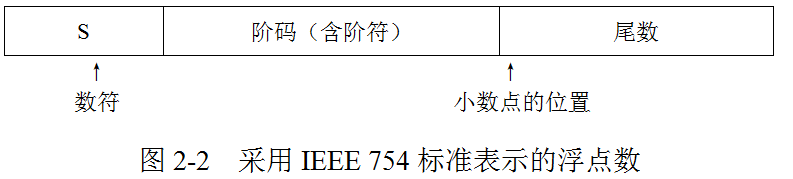
\includegraphics[width=2.80208in,height=0.63542in]{png-jpeg-pics/752F41641C8EDCD76B34C5208BE4D47F.png}

如数符为s,阶码为e,尾数为M

则真值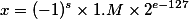
\includegraphics[width=1.96875in,height=0.19792in]{texmath/ccaf64x(-1)stimes1Mtimes2e-127}(32位浮点数)

按照IEEE 754标准,常用的浮点数有以下3种,见下表:

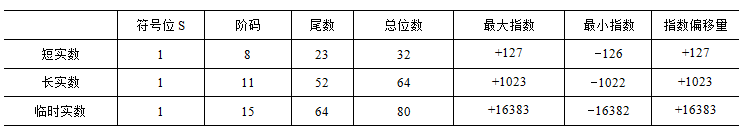
\includegraphics[width=3.69792in,height=0.66667in]{png-jpeg-pics/3D7EB7881E3EFD61FA1063F3DC8A777B.png}
